% -*- program: xelatex -*-

\documentclass[12pt, t]{beamer}
%%% ------------------------------------------------------------------------
% packages
\usepackage{tikz}
\usetikzlibrary{shapes.geometric, arrows, positioning, shapes, backgrounds}
\usepackage{graphicx}
\usepackage{lmodern}
\usepackage{adjustbox}
% conditional (for figures)
\usepackage{etoolbox}
% \usepackage{listings}
\usepackage{minted}

\usepackage{fontspec}
\usepackage{fontawesome}

\usepackage{subcaption} % side-by-side figures
\usepackage{hyperref}



%%% ------------------------------------------------------------------------
% Theming (dark or white)
\usetheme{default}
\useoutertheme[subsection=false]{miniframes}

% move navigation to footer
\setbeamertemplate{headline}{}
\makeatletter
\setbeamertemplate{footline}
  {%
  \begin{beamercolorbox}{section in head/foot}
    \vskip2pt\insertnavigation{\paperwidth}\vskip5pt
  \end{beamercolorbox}%
  }
\makeatother


% no navigation bar
\beamertemplatenavigationsymbolsempty

% switch between white and black
\newtoggle{dark}
\toggletrue{dark}
% \togglefalse{dark}

\iftoggle{dark}{%
    % some colors
    \definecolor{foreground}{RGB}{255,255,255}
    \definecolor{background}{RGB}{24,24,24}
    \definecolor{title}{RGB}{127,185,220}
    \definecolor{gray}{RGB}{154,154,154}
    \definecolor{hilight}{RGB}{250, 108, 0}
    \setbeamercolor{section in head/foot}{fg = title}
    % set colors for titles, etc.
    \setbeamercolor{titlelike}{fg=title}
    \setbeamercolor{subtitle}{fg=title}
    \setbeamercolor{institute}{fg=gray}
    \setbeamercolor{normal text}{fg=foreground,bg=background}
    % % set colors for itemize
    \setbeamercolor{item}{fg=title} % color of bullets
    \setbeamercolor{subitem}{fg=gray}
    \setbeamercolor{itemize/enumerate subbody}{fg=gray}
}{
    % some colors
    \definecolor{foreground}{RGB}{0, 0, 0}
    \definecolor{background}{RGB}{255,255,255}
    \definecolor{title}{RGB}{107,174,214}
    \definecolor{gray}{RGB}{116,116,116}
    \definecolor{hilight}{RGB}{228, 97, 0}
    \setbeamercolor{section in head/foot}{fg = title}
    % set colors
    \setbeamercolor{titlelike}{fg=title}
    \setbeamercolor{subtitle}{fg=title}
    \setbeamercolor{institute}{fg=gray}
    \setbeamercolor{normal text}{fg=foreground,bg=background}
    % set colors for itemize
    \setbeamercolor{item}{fg=foreground} % color of bullets
    \setbeamercolor{subitem}{fg=gray}
    \setbeamercolor{itemize/enumerate subbody}{fg=gray}
}


%%% -----------------------------------------------------------------------


%%% ------------------------------------------------------------------------
% Meta
\title{Web Scraping with R}   
\author{Eduard Szöcs} 
\institute{Institute for Environmental Sciences, UnVersity of Koblenz-Landau} 
\date{Landau, 07.04.2016}



%%% ------------------------------------------------------------------------
% Title page

\begin{document}

\begin{frame}
\vspace*{1.5cm}
\titlepage
\vspace*{1.5cm}
\textcolor{hilight}{\faGift}~~~\textcolor{title}{\href{https://github.com/edild/talk_webscrapingr}{https://github.com/edild/talk\_webscrapingr}}

\end{frame}


%%% ------------------------------------------------------------------------
% Intro
\section{I - About} 
\subsection{}
\begin{frame}
\frametitle{About me}
\begin{itemize}
\item Phd-Student @Uni Koblenz-Landau
	\begin{itemize}
	  \item Environmental data
	\end{itemize}
\item Freelance (R) Consultant
	\begin{itemize}
		\item Data sourcing, cleaning \& analysis
		\item Chemoinformatics
		\item R Courses
	\end{itemize}
\end{itemize}
\pause
\vspace{1.5em}
R packages:
\begin{description}
	\item[\href{https://github.com/ropensci/taxize}{taxize}]{Taxonomic Information from Around the Web}
	\item[\href{https://github.com/ropensci/webchem}{webchem}]{Chemical Information from the Web}
\end{description}
\begin{centering}
\colorbox{white}{
\includegraphics[width =.3\textwidth]{fig/ropensci.png}}
\end{centering}
\end{frame}


\begin{frame}[c]
\frametitle{I What is web scraping?}
\begin{center}
\Huge
\textbf{Getting data from the internet} \\ \pause
\normalsize
\vspace{0.5em}
(in a structured automated way)
\end{center}
\end{frame}



%%% ------------------------------------------------------------------------
% Tools
\section{II - Tools}
\subsection{}
\begin{frame}
\frametitle{II - R Packages for web scraping (selected)}
\begin{description}
\item[\textcolor{hilight}{xml2}]{Parsing HTML \& XML}	
\item[\textcolor{hilight}{rvest}]{parse common html structures (e.g. tables)}
\item[\textcolor{hilight}{xmlview}]{View pretty HTML/XML, explore XPaths}
\item[httr*]{Working with APIs / http protocol}
\item[jsonlite*]{Parse JSON}
\end{description}
\pause

\includegraphics[width=.3\textwidth]{fig/adcr-cover-wiley4.jpg} \\
\tiny
* I won't cover APIs here.
\end{frame}


%%% ------------------------------------------------------------------------
% Structured data
\section{III - Structured data}
\subsection{}
\begin{frame}[fragile]
\frametitle{III - Scraping structured web-pages}
What is structured data?
\vspace{1em}
\begin{minted}[fontsize=\tiny]{html}
<table class="wikitable">
  <tbody>
    <tr>
      <th>First name</th>
      <th>Last name</th>
      <th>Age</th>
    </tr>
    <tr>
      <td>Tinu</td>
      <td>Elejogun</td>
      <td>14</td>
    </tr>
    <tr>
      <td>Blaszczyk</td>
      <td>Kostrzewski</td>
      <td>25</td>
    </tr>
    [...]
  </tbody>
</table>
\end{minted}
2D representation of data -> data.frame
\end{frame}


\begin{frame}
\frametitle{III - Demo}
Extract election results from wikipedia \\
\tiny
\url{https://de.wikipedia.org/wiki/Landtagswahlen_in_Rheinland-Pfalz}

\vspace{1em}
\begin{adjustbox}{max totalsize={.9\textwidth}{.7\textheight},center}
\begin{tikzpicture}[node distance = 1cm, auto]
\tikzstyle{block} = [rectangle, draw, fill=title, text = black,
    text width=8em, text centered, rounded corners, minimum height=4em]
\tikzstyle{line} = [draw, thick, -latex']
    % Place nodes
    \node [block] (source) {Look at the source};
    \node [block, right=of source] (download) {download \\ xml2::read\_html()};
    \node [block, right=of download] (parse) {parse \\ rvest::html\_table()};
    \node [block, right=of parse] (clean) {clean / use};

%paths
    \path [line] (source) -- (download);
    \path [line] (download) -- (parse);
    \path [line] (parse) -- (clean);

\end{tikzpicture}
\end{adjustbox}
\vspace{2em}
\pause
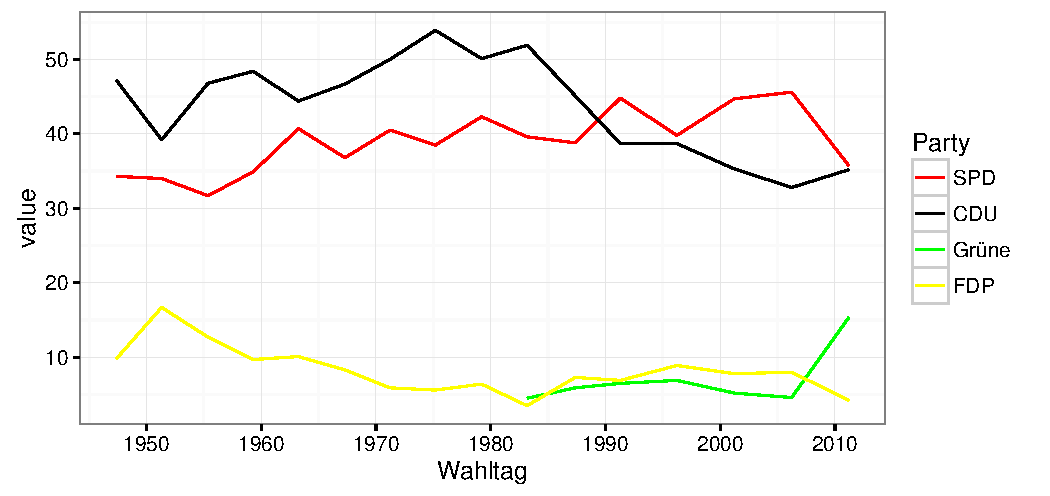
\includegraphics[width=0.7\textwidth]{fig/p1.pdf}
\end{frame}


%%% ------------------------------------------------------------------------
% Unstructured data
\section{IV - Unstructured data}
\subsection{}
\begin{frame}[fragile]
\frametitle{IV - Scraping unstructured web-pages}
\begin{itemize}
	\item Not all data is stored in <table>
	\item scattered on the web page
	\item Need to find and extract the parts we need.
\end{itemize}

\tiny
\url{http://webbook.nist.gov/cgi/cbook.cgi?ID=50-00-0&Units=SI}

	\begin{minted}[fontsize=\tiny]{html}
	<h1 id="Top">Formaldehyde</h1>
	<ul>
	<li>
	<strong>
	<a title="IUPAC definition of relatVe molecular mass (molecular weight)">Molecular weight</a>
	:
	</strong>
	30.0260
	</li>
	<li>
	<strong>IUPAC Standard InChIKey:</strong>
	<span style="font-family: monospace;">WSFSSNUMVMOOMR-UHFFFAOYSA-N</span>
	</li>
	<li>
	<strong>CAS Registry Number:</strong>
	50-00-0
	</li>
	\end{minted}
\end{frame}


\begin{frame}[fragile]
\frametitle{IV - XPath}
\begin{itemize}
  \item XPath is a query language for selecting parts (nodes).
\end{itemize}

\begin{description}
  \item[\textbackslash\textbackslash a]{Select all a elements (links)}
  \item[\textbackslash\textbackslash li\textbackslash a]{Select all links within li}
  \item[\textbackslash\textbackslash li\textbackslash a[3]]{Select third link within li}
\end{description}


\begin{itemize}
  \item Inspectors can export paths (fragile)
  \item Build \textcolor{hilight}{robust} Xpaths
  \item \url{http://www.w3schools.com/xsl/xpath_intro.asp}
\end{itemize}
\end{frame}


\begin{frame}[fragile]
\frametitle{IV - RegEx}
Regular Expressions

\begin{itemize}
  \item For residual cleaning of characters
  \item E.g. Split Value and Unit
  \item gsub() \& Co
  \item \url{http://www.regular-expressions.info}
\end{itemize}
\end{frame}


\begin{frame}
\frametitle{IV - Demo}
Extract Inchikeys from \url{webbook.nist.gov}\\

\vspace{1em}
\begin{adjustbox}{max totalsize={.9\textwidth}{.7\textheight},center}
\begin{tikzpicture}[node distance = 1cm, auto]
\tikzstyle{block} = [rectangle, draw, fill=title, text = black,
    text width=8em, text centered, rounded corners, minimum height=4em]
\tikzstyle{line} = [draw, thick, -latex']
    % Place nodes
    \node [block] (source) {Look at the source / Identify parts};
    \node [block, right=of source] (download) {download \\ xml2::read\_html()};
    \node [block, right=of download] (parse) {XPath \\ xml2::xml\_find\_all()};
    \node [block, right=of parse] (clean) {clean};

%paths
    \path [line] (source) -- (download);
    \path [line] (download) -- (parse);
    \path [line] (parse) -- (clean);

\end{tikzpicture}
\end{adjustbox}


\vspace{1em}
\begin{adjustbox}{max totalsize={.9\textwidth}{.7\textheight},center}
\begin{tikzpicture}[node distance = 1cm, auto]
\tikzstyle{block} = [rectangle, draw, fill=hilight, text = black,
    text width=10em, text centered, rounded corners, minimum height=4em]
\tikzstyle{line} = [draw, thick, -latex']
    % Place nodes
    \node [block] (source) {CAS : 50-00-0};
    \node [block, right=of source] (download) {WSFSSNUMVMOOMR-UHFFFAOYSA-N};

%paths
    \path [line] (source) -- (download);

\end{tikzpicture}
\end{adjustbox}

\end{frame}


%%% ------------------------------------------------------------------------
% Automatisation
\section{V - Automatisation}
\subsection{}

\begin{frame}
  \frametitle{V - Automatisation}
  
  \begin{itemize}
    \item Wrap into function (Input = URL)
    \item Function should return vector or list
    \item Build URLs
    \item Iterate with l/sapply
  \end{itemize}

\end{frame}

\begin{frame}
  \frametitle{V - Demo Automatisation}
  \begin{adjustbox}{max totalsize={.9\textwidth}{.7\textheight},center}
  \begin{tikzpicture}[node distance = 1cm, auto]
  \tikzstyle{block} = [rectangle, draw, fill=title, text = black,
      text width=8em, text centered, rounded corners, minimum height=4em]
  \tikzstyle{line} = [draw, thick, -latex']
      % Place nodes
      \node [block] (source) {Input};
      \node [block, right=of source] (download) {Build URL};
      \node [block, right=of download] (parse) {Apply Function to URL};
      \node [block, right=of parse] (clean) {Combine};
  
  %paths
      \path [line] (source) -- (download);
      \path [line] (download) -- (parse);
      \path [line] (parse) -- (clean);
  
  \end{tikzpicture}
  \end{adjustbox}
  
\vspace{1em}
\begin{table}[htbp]
\footnotesize
\begin{tabular}{llr}
CAS & inchikey & \multicolumn{1}{l}{mw} \\ \hline
50-00-0 & WSFSSNUMVMOOMR-UHFFFAOYSA-N & 30.026 \\ 
126-86-3 & LXOFYPKXCSULTL-UHFFFAOYSA-N & 226.355 \\ 
28159-98-0 & HDHLIWCXDDZUFH-UHFFFAOYSA-N & 253.367 \\ 
1461-25-2 & AFCAKJKUYFLYFK-UHFFFAOYSA-N & 347.167 \\ 
120-18-3 &  & \multicolumn{1}{l}{} \\ 
25637-99-4 &  & \multicolumn{1}{l}{} \\ \hline
\end{tabular}
\label{}
\end{table}

\end{frame}


%%% ------------------------------------------------------------------------
% Conclusions
\section{VI - Conclusions}
\subsection{}

\begin{frame}
  \frametitle{VI - Remarks}
  \begin{itemize}
  	\item Error handling?
  	\item Robustness? (e.g. Change in website)
  	\item APIs! (functions provided by servers to query data)
  	\item ROpenSci (e.g. \href{https://github.com/ropensci/webchem}{webchem}) provides good functionalities
  	\item \url{forum.r-statistik.de}
  \end{itemize}
\end{frame}

\begin{frame}
  \frametitle{VI - Lessons learned}
  \begin{itemize}
  	\item scraping is easy.
  	\item being user-friendly is \textcolor{hilight}{not}.
  	\item be nice to the servers!
  	\begin{itemize}
  		\item scrape slowly, time-outs
  		\item Sys.sleep(rgamma(1, shape = 30, scale = 1/10))
  	\end{itemize}
  	\item legal?
  	\begin{itemize}
  		\item even slower
  		\item anonymous EC2
  		\item TOR
  	\end{itemize}
  \end{itemize}
\end{frame}



%%% Last slide ----------------------------------------------------
\begin{frame}
    \frametitle{}

    \vspace{1em}
    \begin{centering}
    \Large \textcolor{title}{Web Scraping with R} \\[1em]
        Eduard Szöcs \\[0.3em]
    \tiny \textcolor{gray}{Institute for Environmental Sciences, UnVersity of Koblenz-Landau} \\[5em]
    \end{centering}
    \normalsize
    \textcolor{hilight}{\faLaptop}~~~\href{http://edild.github.io/}{http://edild.github.io/ }\\[.5em]
    \textcolor{hilight}{\faGift}~~~\href{https://github.com/edild/talk_webscrapingr}{https://github.com/edild/talk\_webscrapingr}\\[0.5em]
    \textcolor{hilight}{\faTwitter}~~~\href{http://twitter.com/EduardSzoecs}{@EduardSzoecs}     \\[0.5em]
    \textcolor{hilight}{\faEnvelope}~~~\href{mailto:szoecs@uni-landau.de}{szoecs@uni-landau.de} \\[.5em]
    \hfill 
\includegraphics[width =.3\textwidth]{fig/Cc-by-nc_euro_icon.png} 
\end{frame}


\end{document}
